% id: 0499
% book: RPM 중3-2 수학 · 04 원주각
% section: 중단원 마무리하기
% figure: crop:fig-0499.png
% answer: ①
% answer_source: 답지
% variant_level: 0 (원본 전사)
% 이 파일은 build.mjs 가 items.json 에서 만든다. 고칠 때는 items.json 을 고친다.
\noindent\begin{minipage}[t]{0.58\linewidth}\vspace{0pt}\raggedright 오른쪽 그림과 같이 원~$\pt{O}$에 내접하는 $\triangle\pt{ABC}$에서 $\angle\pt{BAC}=60^\circ$ $\seg{BC}=2\sqrt{3}\mkern3mu \mathrm{cm}$일 때, 원~$\pt{O}$의 지름의 길이는?\end{minipage}\hfill\begin{minipage}[t]{0.4\linewidth}\vspace{0pt}\centering \setlength{\dmfigw}{69.2pt}\ifdim\dmfigw>\linewidth\setlength{\dmfigw}{\linewidth}\fi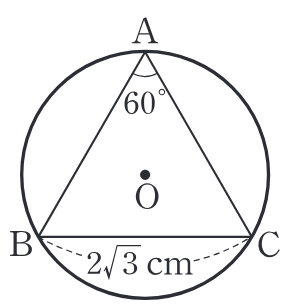
\includegraphics[width=\dmfigw]{figures/fig-0499.png}\end{minipage}\par
\begin{choicesii}{\rule[-3ex]{0pt}{8ex}$4\mkern3mu \mathrm{cm}$}{\rule[-3ex]{0pt}{8ex}$3\sqrt{2}\mkern3mu \mathrm{cm}$}{\rule[-3ex]{0pt}{8ex}$3\sqrt{3}\mkern3mu \mathrm{cm}$}{\rule[-3ex]{0pt}{8ex}$2\sqrt{7}\mkern3mu \mathrm{cm}$}{\rule[-3ex]{0pt}{8ex}$4\sqrt{2}\mkern3mu \mathrm{cm}$}\end{choicesii}
